\renewcommand{\thetheorem}{4.\arabic{theorem}}
\setcounter{theorem}{0}
\setcounter{chapter}{3}

\chapter{Maps}

\subsection{Functions and their Domains}

\begin{definition}[Map / Function]
Let $X$ and $Y$ be sets. A map $f: X \to Y$ (also called a function or transformation) is an assignment that assigns to every element $x \in X$ a uniquely defined element $f(x) \in Y$. 
\end{definition}

In accordance with this definition, we can visually distinguish between valid and invalid assignments. A function must assign exactly one output to each input in its domain.

\begin{center}
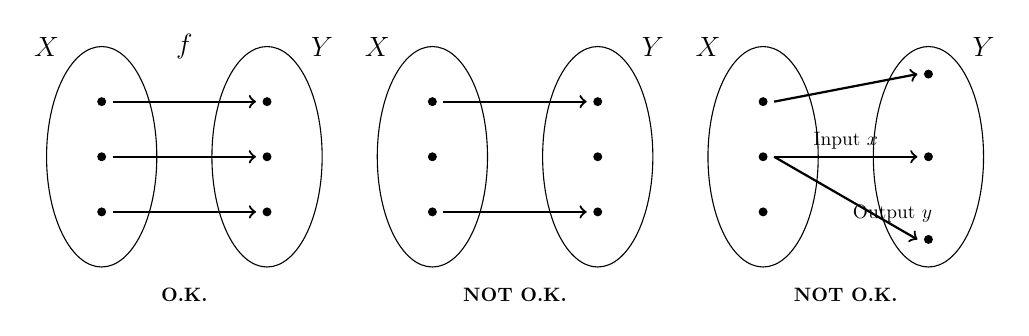
\begin{tikzpicture}[scale=0.7, every node/.style={transform shape}]
    % Diagram 1: O.K.
    \begin{scope}[shift={(0,0)}]
        \draw (0,0) ellipse (1cm and 2cm); \node at (-1, 2) {\Large $X$};
        \draw (3,0) ellipse (1cm and 2cm); \node at (4, 2) {\Large $Y$};
        \filldraw (0, 1) circle (2pt); \filldraw (0, 0) circle (2pt); \filldraw (0, -1) circle (2pt);
        \filldraw (3, 1) circle (2pt); \filldraw (3, 0) circle (2pt); \filldraw (3, -1) circle (2pt);
        \draw[->, thick] (0.2, 1) -- (2.8, 1);
        \draw[->, thick] (0.2, 0) -- (2.8, 0);
        \draw[->, thick] (0.2, -1) -- (2.8, -1);
        \node at (1.5, -2.5) {\textbf{O.K.}};
        \node at (1.5, 2) {\Large $f$};
    \end{scope}

    % Diagram 2: NOT O.K. (Undefined for some x)
    \begin{scope}[shift={(6,0)}]
        \draw (0,0) ellipse (1cm and 2cm); \node at (-1, 2) {\Large $X$};
        \draw (3,0) ellipse (1cm and 2cm); \node at (4, 2) {\Large $Y$};
        \filldraw (0, 1) circle (2pt); \filldraw (0, 0) circle (2pt); \filldraw (0, -1) circle (2pt);
        \filldraw (3, 1) circle (2pt); \filldraw (3, 0) circle (2pt); \filldraw (3, -1) circle (2pt);
        \draw[->, thick] (0.2, 1) -- (2.8, 1);
        % The middle element in X has no output arrow!
        \draw[->, thick] (0.2, -1) -- (2.8, -1);
        \node at (1.5, -2.5) {\textbf{NOT O.K.}};
    \end{scope}

    % Diagram 3: NOT O.K. (Multiple outputs for one x)
    \begin{scope}[shift={(12,0)}]
        \draw (0,0) ellipse (1cm and 2cm); \node at (-1, 2) {\Large $X$};
        \draw (3,0) ellipse (1cm and 2cm); \node at (4, 2) {\Large $Y$};
        \filldraw (0, 1) circle (2pt); \filldraw (0, 0) circle (2pt); \filldraw (0, -1) circle (2pt);
        \filldraw (3, 1.5) circle (2pt); \filldraw (3, 0) circle (2pt); \filldraw (3, -1.5) circle (2pt);
        
        \draw[->, thick] (0.2, 1) -- (2.8, 1.5);
        \draw[->, thick] (0.2, 0) -- (2.8, 0) node[midway, above] {Input $x$};
        \draw[->, thick] (0.2, 0) -- (2.8, -1.5) node[midway, below right] {Output $y$};
        \node at (1.5, -2.5) {\textbf{NOT O.K.}};
    \end{scope}
\end{tikzpicture}
\end{center}

$X$ is called the \textit{domain of definition} of $f$. 
$Y$ is called the \textit{target} (or target domain) of $f$.

\begin{definition}[Equality of Functions]
Two functions $f: X \to Y$ and $g: X' \to Y'$ are equal if they have the same domain of definition ($X' = X$), the same target ($Y' = Y$), and for all $x \in X$, we have $f(x) = g(x)$.
\end{definition}

Sometimes a function is given by a formula, and sometimes it is not. Be careful: providing just a formula is often mathematically insufficient.

\begin{example}[Specifying Domain and Target]
\textbf{Bad notation:} $f(x) = x^2$. (What are the domain and target?)

\textbf{O.K. notation:} Let $X := \{x \in \mathbb{R} \mid 0 \le x\}$. Define $f: X \to \mathbb{R}$ by $f(x) = x^2$.
\end{example}

\begin{example}[Student Database Function]
Let $X = \{x \in \mathbb{Z} \mid x \ge 0\}$ and let $Y$ be the set of family names. We might try to define a map $g: X \to Y$ by setting $g(x)$ to be the family name of the student at ETH whose student number is $x$.

This $g$ is \textbf{not} defined! What is $g(0)$? What is $g(10^{10})$? There are no students with these IDs. 

To fix this, we could define $Y' = Y \cup \{\text{ERROR!}\}$ and introduce a rigorous function $h: X \to Y'$ given by:
\[
h(x) = 
\begin{cases} 
\text{family name} & \text{if a student with student no. } x \text{ exists} \\
\text{ERROR!} & \text{otherwise}
\end{cases}
\]
\end{example}

\begin{remark}
\textbf{Notation:} We frequently use the barred arrow ($\mapsto$) to denote how individual elements are mapped. For example, $f: X \to Y, X \ni x \mapsto f(x) \in Y$. 
Concretely: $f: \mathbb{R} \to \mathbb{R}, \mathbb{R} \ni x \mapsto x^5 \in \mathbb{R}$.
\end{remark}

\subsection{Images and Restrictions}

\begin{definition}[Image of a Map]Let $f: X \to Y$ be a map. The \textit{image} of $f$ is the set:
\[
f(X) := \{y \in Y \mid \exists x \in X \text{ s.t. } f(x) = y\}
\]
(sometimes written as $\text{image}(f)$). Clearly, $f(X) \subseteq Y$.
\end{definition}

\begin{definition}[Restriction and Extension]
Let $f: X \to Y$ be a map, and let $A \subseteq X$ be a subset. We can define a new map $f|_A: A \to Y$, called the \textit{restriction} of $f$ to $A$, simply by $f|_A(x) := f(x)$ for all $x \in A$.
Conversely, $f$ is called an \textit{extension} of $f|_A$.
\end{definition}

\subsection{Some Standard Maps}

\begin{example}[Standard Maps]
\begin{enumerate}
    \item \textbf{Identity Map:} $\id: X \to X$ (sometimes denoted $\id_X$), defined by $\id(x) = x$ for all $x \in X$.
    \item \textbf{Constant Map:} $f: X \to Y$. Choose a fixed $y_0 \in Y$. Then $f(x) = y_0$ for all $x \in X$.
    \item \textbf{Characteristic Function:} Let $A \subseteq X$. The characteristic function $\chi_A: X \to \{0, 1\}$ is defined as:
    \[
    \chi_A(x) = 
    \begin{cases}
    1 & \text{if } x \in A \\
    0 & \text{if } x \notin A
    \end{cases}
    \]
    \item \textbf{Projections:} Given a Cartesian product $X_1 \times X_2$, the standard projection maps are:
    \begin{align*}
    p_1&: X_1 \times X_2 \to X_1, \quad p_1(x_1, x_2) = x_1 \\
    p_2&: X_1 \times X_2 \to X_2, \quad p_2(x_1, x_2) = x_2
    \end{align*}
\end{enumerate}
\end{example}

\subsection{Injectivity, Surjectivity, Bijectivity}

\begin{definition}[Injectivity, Surjectivity, and Bijectivity]
Let $f: X \to Y$ be a map.
\begin{enumerate}
    \item We say $f$ is \textbf{injective} if $\forall x_1, x_2 \in X$, $f(x_1) = f(x_2) \implies x_1 = x_2$. (Equivalently, by contrapositive: $x_1 \ne x_2 \implies f(x_1) \ne f(x_2)$).
    \item We say $f$ is \textbf{surjective} if $\forall y \in Y, \exists x \in X$ such that $f(x) = y$. (Equivalently: $f(X) = Y$).
    \item We say $f$ is \textbf{bijective} (or a \textit{bijection}) if $f$ is both injective and surjective. (Equivalently: $\forall y \in Y, \exists! x \in X : f(x) = y$).
\end{enumerate}
\end{definition}

\begin{example}[Injective and Surjective Squaring Functions]
Consider variations of the squaring function, which explicitly demonstrate the importance of the chosen domain and target:
\begin{itemize}
    \item $f: \mathbb{R} \to \mathbb{R}, f(x) = x^2$. Not injective (e.g., $f(2) = f(-2)$). Not surjective (no real $x$ maps to $-1$).
    \item $f: \mathbb{R}_{\ge 0} \to \mathbb{R}, f(x) = x^2$. Injective, but not surjective.
    \item $f: \mathbb{R}_{\ge 0} \to \mathbb{R}_{\ge 0}, f(x) = x^2$. Bijective.
\end{itemize}
\end{example}

\begin{definition}[Inverse Map]
Let $f: X \to Y$ be a bijection. The \textit{inverse map} $f^{-1}: Y \to X$ is the map that assigns to every $y \in Y$ the unique $x \in X$ such that $f(x) = y$.
\end{definition}

\begin{center}
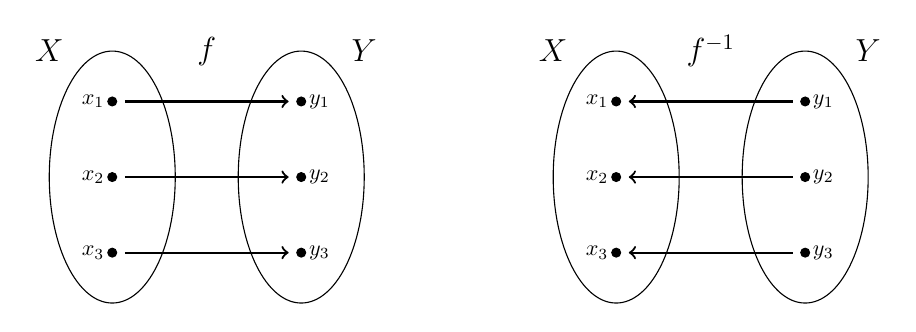
\begin{tikzpicture}[scale=0.8, every node/.style={transform shape}]
    % Forward Map f
    \begin{scope}[shift={(0,0)}]
        \draw (0,0) ellipse (1cm and 2cm); \node at (-1, 2) {\Large $X$};
        \draw (3,0) ellipse (1cm and 2cm); \node at (4, 2) {\Large $Y$};
        \filldraw (0, 1.2) circle (2pt) node[left] {$x_1$};
        \filldraw (0, 0) circle (2pt) node[left] {$x_2$};
        \filldraw (0, -1.2) circle (2pt) node[left] {$x_3$};
        \filldraw (3, 1.2) circle (2pt) node[right] {$y_1$};
        \filldraw (3, 0) circle (2pt) node[right] {$y_2$};
        \filldraw (3, -1.2) circle (2pt) node[right] {$y_3$};
        \draw[->, thick] (0.2, 1.2) -- (2.8, 1.2);
        \draw[->, thick] (0.2, 0) -- (2.8, 0);
        \draw[->, thick] (0.2, -1.2) -- (2.8, -1.2);
        \node at (1.5, 2) {\Large $f$};
    \end{scope}
    
    % Inverse Map f^{-1}
    \begin{scope}[shift={(8,0)}]
        \draw (0,0) ellipse (1cm and 2cm); \node at (-1, 2) {\Large $X$};
        \draw (3,0) ellipse (1cm and 2cm); \node at (4, 2) {\Large $Y$};
        \filldraw (0, 1.2) circle (2pt) node[left] {$x_1$};
        \filldraw (0, 0) circle (2pt) node[left] {$x_2$};
        \filldraw (0, -1.2) circle (2pt) node[left] {$x_3$};
        \filldraw (3, 1.2) circle (2pt) node[right] {$y_1$};
        \filldraw (3, 0) circle (2pt) node[right] {$y_2$};
        \filldraw (3, -1.2) circle (2pt) node[right] {$y_3$};
        \draw[<-, thick] (0.2, 1.2) -- (2.8, 1.2);
        \draw[<-, thick] (0.2, 0) -- (2.8, 0);
        \draw[<-, thick] (0.2, -1.2) -- (2.8, -1.2);
        \node at (1.5, 2) {\Large $f^{-1}$};
    \end{scope}
\end{tikzpicture}
\end{center}

\begin{example}[Inverse of Squaring Function]
For the bijection $f: \mathbb{R}_{\ge 0} \to \mathbb{R}_{\ge 0}$ with $f(x) = x^2$, the inverse map is $f^{-1}: \mathbb{R}_{\ge 0} \to \mathbb{R}_{\ge 0}$, strictly defined by $f^{-1}(y) = \sqrt{y}$.
\end{example}

\subsection{Composition of Maps}

\begin{definition}[Composition]
Let $f: X \to Y$ and $g: Y \to Z$ be maps. The composition $g \circ f: X \to Z$ is defined by:
\[
(g \circ f)(x) := g(f(x))
\]
\end{definition}

\begin{example}[Composition with Inverse]
If $f: X \to Y$ is bijective and $f^{-1}: Y \to X$ is its inverse, then by definition:
\[
f^{-1} \circ f = \id_X \quad \text{and} \quad f \circ f^{-1} = \id_Y
\]
\end{example}

\begin{remark}
If $g \circ f$ is defined, $f \circ g$ is in general NOT defined (unless $Z=X$). But even when $Z=X$, in general $g \circ f \ne f \circ g$. Commutativity is not guaranteed.
\end{remark}

\begin{example}[Non-Commutative Compositions]
Let $f, g: \mathbb{R} \to \mathbb{R}$ with $f(x) = x^2$ and $g(x) = x+1$.
\begin{align*}
(g \circ f)(x) &= g(x^2) = x^2 + 1 \\
(f \circ g)(x) &= f(x+1) = (x+1)^2 = x^2 + 2x + 1
\end{align*}
Clearly, $g \circ f \ne f \circ g$.
\end{example}

\begin{lemma}[Composition of Injective and Surjective Maps]
Let $f: X \to Y$ and $g: Y \to Z$ be maps.
\begin{enumerate}[label=\textbf{(\alph*)}]
    \item If $f$ and $g$ are injective, then $g \circ f$ is injective.
    \item If $f$ and $g$ are surjective, then $g \circ f$ is surjective.
\end{enumerate}
\end{lemma}

\begin{proof}
\begin{enumerate}[label=\textbf{(\alph*)}]
    \item Assume $f$ and $g$ are injective. Let $x_1, x_2 \in X$ such that $(g \circ f)(x_1) = (g \circ f)(x_2)$. This means $g(f(x_1)) = g(f(x_2))$. Because $g$ is injective, this implies $f(x_1) = f(x_2)$. Because $f$ is injective, this implies $x_1 = x_2$. Thus, $g \circ f$ is injective.
    \item Assume $f$ and $g$ are surjective. Let $z \in Z$. Because $g$ is surjective, there exists $y \in Y$ such that $g(y) = z$. Because $f$ is surjective, there exists $x \in X$ such that $f(x) = y$. Therefore, $g(f(x)) = g(y) = z$, which means $(g \circ f)(x) = z$. Thus, $g \circ f$ is surjective.
\end{enumerate}
\end{proof}

\subsection{Visualizing Properties via Graphs}

We can often immediately determine the injectivity, surjectivity, and bijectivity of a function—or whether an assignment is a function at all—by examining its Cartesian graph using horizontal and vertical line tests.

\begin{center}
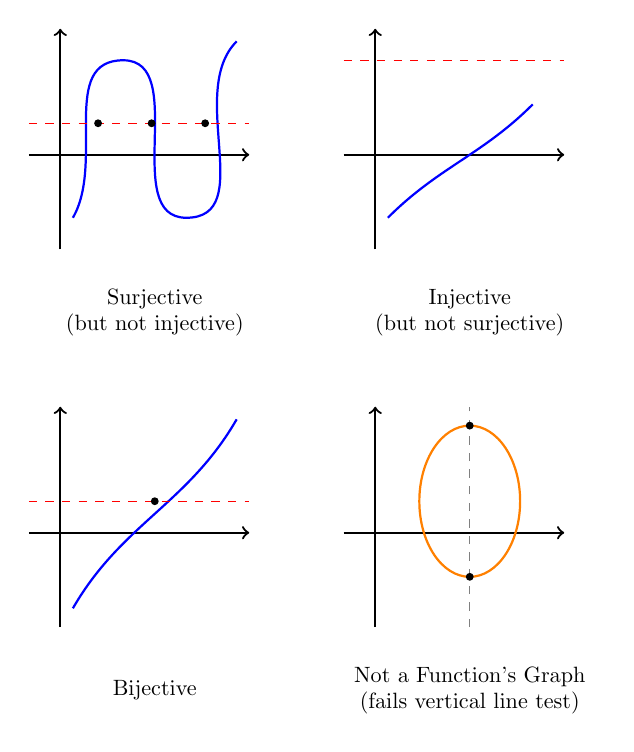
\begin{tikzpicture}[scale=0.8, every node/.style={transform shape}]
    % Surjective, but not injective
    \begin{scope}[shift={(0,0)}]
        \draw[->, thick] (-0.5,0) -- (3,0);
        \draw[->, thick] (0,-1.5) -- (0,2);
        \draw[thick, blue] (0.2,-1) to[out=60, in=180] (1, 1.5) to[out=0, in=180] (2, -1) to[out=0, in=225] (2.8, 1.8);
        \draw[dashed, red] (-0.5, 0.5) -- (3, 0.5);
        \filldraw (0.6, 0.5) circle (1.5pt);
        \filldraw (1.45, 0.5) circle (1.5pt);
        \filldraw (2.3, 0.5) circle (1.5pt);
        \node at (1.5, -2.5) {\begin{tabular}{c} Surjective \\ (but not injective) \end{tabular}};
    \end{scope}

    % Injective, but not surjective
    \begin{scope}[shift={(5,0)}]
        \draw[->, thick] (-0.5,0) -- (3,0);
        \draw[->, thick] (0,-1.5) -- (0,2);
        \draw[thick, blue] (0.2,-1) to[out=45, in=225] (2.5, 0.8);
        \draw[dashed, red] (-0.5, 1.5) -- (3, 1.5);
        \node at (1.5, -2.5) {\begin{tabular}{c} Injective \\ (but not surjective) \end{tabular}};
    \end{scope}

    % Bijective
    \begin{scope}[shift={(0,-6)}]
        \draw[->, thick] (-0.5,0) -- (3,0);
        \draw[->, thick] (0,-1.5) -- (0,2);
        \draw[thick, blue] (0.2,-1.2) to[out=60, in=240] (2.8, 1.8);
        \draw[dashed, red] (-0.5, 0.5) -- (3, 0.5);
        \filldraw (1.5, 0.5) circle (1.5pt);
        \node at (1.5, -2.5) {\begin{tabular}{c} Bijective \end{tabular}};
    \end{scope}

    % NOT a graph (fails vertical line test)
    \begin{scope}[shift={(5,-6)}]
        \draw[->, thick] (-0.5,0) -- (3,0);
        \draw[->, thick] (0,-1.5) -- (0,2);
        \draw[thick, orange] (1.5, 0.5) ellipse (0.8cm and 1.2cm);
        \draw[dashed, gray] (1.5, -1.5) -- (1.5, 2);
        \filldraw (1.5, -0.7) circle (1.5pt);
        \filldraw (1.5, 1.7) circle (1.5pt);
        \node at (1.5, -2.5) {\begin{tabular}{c} Not a Function's Graph \\ (fails vertical line test) \end{tabular}};
    \end{scope}
\end{tikzpicture}
\end{center}

\subsection{Image and Inverse Image of Subsets}

\begin{definition}[Image of a Subset]Let $f: X \to Y$ be a map, and let $A \subseteq X$. The \textit{image of $A$ under $f$} is:
\[
f(A) := \{y \in Y \mid \exists x \in A \text{ s.t. } f(x) = y\} = \{f(x) \mid x \in A\}
\]
\end{definition}

\begin{definition}[Inverse Image of a Subset]
Let $f: X \to Y$ be a map, and let $B \subseteq Y$. The \textit{inverse image of $B$ under $f$} is:
\[
f^{-1}(B) := \{x \in X \mid f(x) \in B\} \subseteq X
\]
\end{definition}

\begin{importantremark}
The notation $f^{-1}(B)$ is somewhat confusing, as this set exists and is perfectly well-defined even if the map $f$ is not invertible!
\end{importantremark}

\begin{example}[Preimages of Subsets]
Consider $f: \mathbb{R} \to \mathbb{R}, f(x) = x^2$ (which is neither injective nor surjective). We can still compute inverse images of subsets without issue:
\begin{align*}
f^{-1}(\{4\}) &= \{-2, 2\} \\
f^{-1}(\{1, 9\}) &= \{-1, 1, -3, 3\} \\
f^{-1}(\{0\}) &= \{0\} \\
f^{-1}(\{-1\}) &= \emptyset \\
f^{-1}(\{-1, 0\}) &= \{0\}
\end{align*}
\end{example}

\subsection{Partitions}

\begin{definition}[Partition]
Let $X$ be a set and $\mathcal{P}$ a family of subsets of $X$, none of which is empty. We say that $\mathcal{P}$ is a \textit{partition} of $X$ if the following hold:
\begin{enumerate}
    \item $X = \bigcup_{P \in \mathcal{P}} P$ (the subsets cover $X$).
    \item For any $P_1, P_2 \in \mathcal{P}$ with $P_1 \ne P_2$, we have $P_1 \cap P_2 = \emptyset$ (the subsets are mutually disjoint).
\end{enumerate}
\end{definition}

\begin{center}
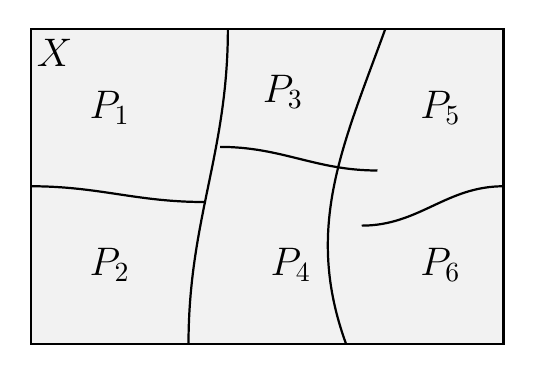
\begin{tikzpicture}[scale=1]
    % Outer set X
    \draw[thick, fill=gray!10] (0,0) rectangle (6,4);
    \node at (0.3, 3.7) {\Large $X$};
    
    % Partition lines
    \draw[thick] (2,0) to[out=90, in=270] (2.5,4);
    \draw[thick] (4,0) to[out=110, in=250] (4.5,4);
    \draw[thick] (0, 2) to[out=0, in=180] (2.2, 1.8);
    \draw[thick] (2.4, 2.5) to[out=0, in=180] (4.4, 2.2);
    \draw[thick] (4.2, 1.5) to[out=0, in=180] (6, 2);
    
    % Labels
    \node at (1, 3) {\Large $P_1$};
    \node at (1, 1) {\Large $P_2$};
    \node at (3.2, 3.2) {\Large $P_3$};
    \node at (3.3, 1) {\Large $P_4$};
    \node at (5.2, 3) {\Large $P_5$};
    \node at (5.2, 1) {\Large $P_6$};
\end{tikzpicture}
\end{center}
